% 2010 年北京卷理科第 12 题：圆 O 的两条割线 ADE、ACB 交于 A，BD⊥AE。
% 来源 PDF：普通高考/2010/2010北京理.pdf，SHA-256 6b5819672aaf59aecfce92e08c2d045a80575803527d61813497dd669a8d5529。
% 原页：第 1 页（A3 三栏）第 3 栏中部，书页码 573。
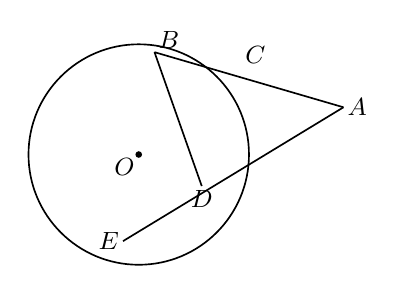
\begin{tikzpicture}[semithick, every node/.style={inner sep=1.2pt, font=\small}]
  \draw (0,0) circle (1.4);
  \coordinate (O) at (0,0);
  \coordinate (A) at (2.6,0.6);
  % 割线 A-D-E
  \coordinate (D) at (0.8,-0.4);
  \coordinate (E) at (-0.2,-1.1);
  % 割线 A-C-B
  \coordinate (C) at (1.3,1.1);
  \coordinate (B) at (0.2,1.3);
  \draw (A) -- (E);
  \draw (A) -- (B);
  \draw (B) -- (D);
  \fill (O) circle (1.2pt);
  \node[below left] at (O) {$O$};
  \node[right] at (A) {$A$};
  \node[above right] at (B) {$B$};
  \node[above right] at (C) {$C$};
  \node[below] at (D) {$D$};
  \node[left] at (E) {$E$};
\end{tikzpicture}
